\documentclass[a4paper]{article}

\usepackage[left=30mm,right=30mm,top=30mm,bottom=30mm]{geometry}
\usepackage[english]{babel}
\usepackage[utf8]{inputenc}
\usepackage{amsmath,amssymb}
\usepackage{multirow}
\usepackage{graphicx}
\usepackage{cite}
\usepackage{hyperref}

\title{COMP5212 Machine Learning 2018 Fall Programming Project \\
       \ \ \ \ \\
       Building Self-driving Agents with Various Deep Learning Methods}

\author{Hok Chun Ng, 20272532, hcngac@connect.ust.hk \\
        Shengyuan Zhang, 20565161, szhangcg@connect.ust.hk \\
        Ge Chen, 20360858, gchenaj@connect.ust.hk}

\date{\today}

\begin{document}
\maketitle

\begin{abstract}
In this project, we build self-driving agents that only rely on vision using various deep learning algorithms: supervised CNN, deep Q learning\cite{mnih2015human} and deep deterministic policy gradient\cite{silver2014deterministic}. Due to the limitations of real-world hardware and data, we use an open source self-driving car simulator provided by Udacity \cite{selfdrivingsimulator} to generate training data and testing platform. We generated human-driving data for training of supervised CNN, and we implemented and ran the two deep-reinforcement algorithms on the car simulator. We evaluated the results of the three algorithms, discovering that only supervised CNN model can smoothly drive the car simulator.
\end{abstract}

\section{Application and practical significance}

Self-driving car has been a hot topic in recent years. Several industry giants, such as Google
\cite{waymo} and Tesla Motor \cite{tesla}, have devoted significant efforts to the developing of
self-driving cars. 

Applications of self-driving agent can be wide. Example includes long-distance truck driving,
smart taxi and bus, or even be incorporated into large-scale autonomous traffic systems.

Letting computers to drive can release human beings from the boring and tiring job of driving as
well as reduce the frequency of traffic accidents. It also opens up new business and
city-management opportunities including smart traffic system and smart taxi services.
Applications are wide and undiscovered and the significance of perfecting self-driving agent is
huge in opening the door to these huge possibilities.

However, designing a robust self-driving system is non-trivial as the real-world traffic
conditions are diverse. Limited by hardware requirement and law, we try to find a solution to
self-driving in a simulated game environment in the hope that the result can be transferred to
real-world self-driving.


\section{Problem formulation}

We formulate the problem of self-driving as a Markov Decision Process. The self-driving agent receives input from front camera and choose the optimal car control according to the input. Each and every image input depends on all previous states and actions from start, so the optimal action to be chosen also depends on all the previous states and actions.

For human drivers, the driving behaviour can be formulated in a loop from an environment sensing
input to action output. Our eyes and ears are the sensors to interpret the current environment,
including the road view from wind screen (e.g. weather, traffic lights, walking people), view
from side mirror (e.g. neighboring cars, following cars), car horns, and so on. Then our brain
takes all these input signals to decide what action to take, including turning the
steering wheel, lighting turn signals, accelerating, braking, and so on. Once the actions are
executed, the environment input changes, and drivers will decide and take a new round of
actions accordingly. This loop continues until the car arrives at the destination. 

We try to mimic how human decision works with machine learning algorithms within a simplified car simulator environment. The machine learning problem in self-driving is: given a camera image input, find the optimal steering angle to turn, in order to drive along the track for as long as possible.


\section{Udacity Self-driving car simulator}

In this project, we develop our algorithms to drive an open source self-driving car simulator provided by Udacity \cite{selfdrivingsimulator}. The simulator provides a near real-world environment of a racing car and a track. The simulator provides image and status data of every frame instances. The expected frame frequency is 30 frames per second. There are two modes in the simulator, one is ``Training mode'' for human controlled training records and the other is ``Autonomous mode'' for training by a machine agent. We record human driving experience (image input and corresponding human action) from ``Training mode'' as training data for supervised learning. We let reinforcement learning algorithms to explore ``Autonomous mode'' freely. A part of the official behavioral cloning skeleton repository \cite{carndbehavioralcloning} provides the facility to interact with the simulation environment. 

The controls to the car include the steering angle and the throttle value. The steering angle of real values from $-1$ to $1$ degrees. The throttle value ranges from $0$ to $1$. To simplify the control, we set throttle value constantly to $1$ and apply the steering angle control. The highest speed in simulation is 30 miles per hour and the end of a simulation is caused by a sudden decrease of car speed.

A sample image during training is shown in Figure \ref{fig:sample_rgb}, which is similar to a front view during human driving. The images are $320 \times 160$ RGB images. To reduce training overhead, we convert the RGB images to gray-scale. After observing the sample images, we find that the gray-scale image data for the Red channel has better information for acting later on. 

\begin{figure}
    \centering
    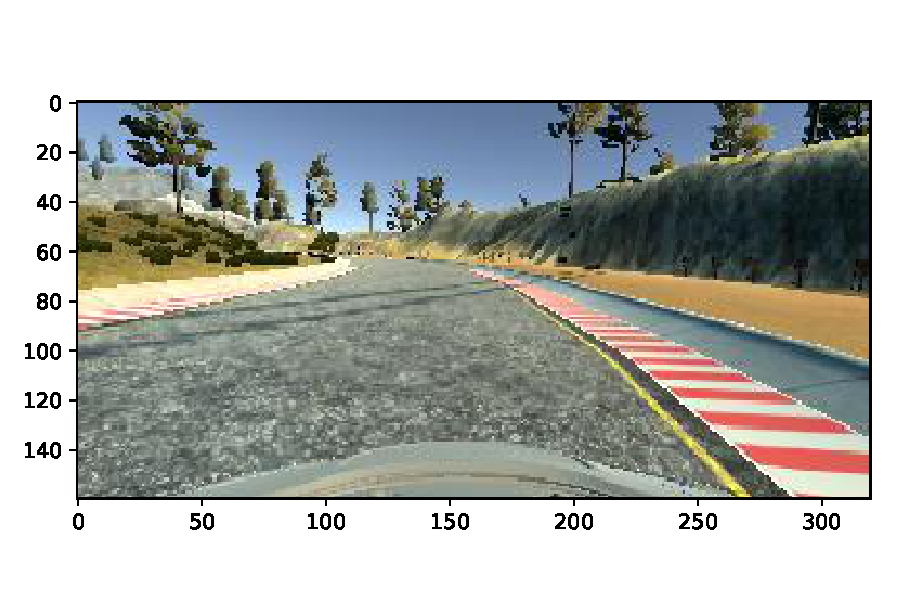
\includegraphics[width=0.8\textwidth]{./figures/sample_rgb.pdf}
    \caption{ Sample image generated by the Udacity simulator }
    \label{fig:sample_rgb}
\end{figure}


\section{Machine learning methods}

In this project, we explore the possibility of using supervised CNN, deep Q learning\cite{mnih2015human} with discrete action space and deep deterministic policy gradient\cite{lillicrap2015continuous} to train a self-driving agent.

\subsection{Supervised CNN}

Supervised learning of CNN creates a model that can recognize imagery input and gives appropriate output accordingly. In our situation, the CNN model solves the regression. The model creates an approximation to the input image - action pair provided by human driving experience, thus approximating human driving.

\subsection{Reinforcement learning}
The environment-action loop in the driving experience resembles the basics of reinforcement learning, an area of machine learning concerned with taking actions according to state of an environment in order to maximize some notion of cumulative reward, as illustrated in Fig. \ref{fig:RL}. Reinforcement learning does not require labeled data as in supervised learning. Instead, reinforcement learning requires a reward feedback from the environment. For driving, the final reward can be no traffic accident and arrive at the destination safely, which translates to no sudden decrease in speed.

\begin{figure}
    \centering
    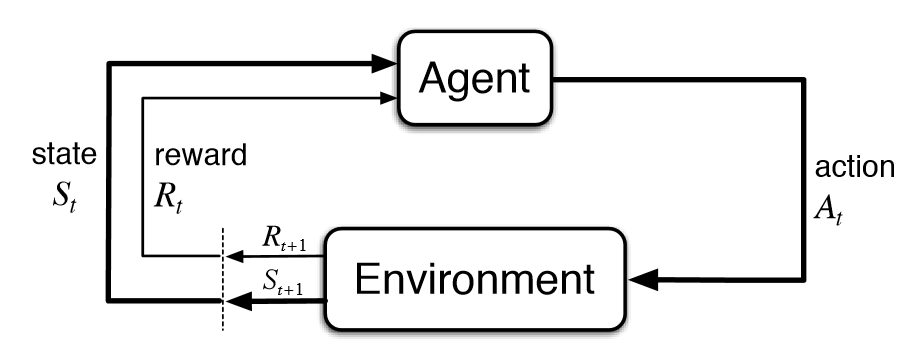
\includegraphics[width=0.8\textwidth]{./figures/rl.png}
    \caption{ Reinforcement Learning Illustration \cite{sutton2018reinforcement}}
    \label{fig:RL}
\end{figure}


Figure \ref{fig:RL} shows the basic model of reinforcement learning \cite{sutton2018reinforcement}. At
each time $t$, an agent receives the environment state $S_t \in \mathcal{S}$ and current scalar
reward $R_t$. It then chooses an action $a_t \in \mathbb{R}^N$ from the set of available
actions, which is sent to the environment. 

The environment moves to a new state $S_{t+1}$ and new reward $R_{t+1}$ and feedback to the agent.
The goal of a reinforcement learning agent is to gain as much as reward as possible. A policy
$\pi$ is defined to map states to a probability distribution over the actions $\pi : \mathcal{S}
\ \rightarrow\ \mathcal{P}(\mathcal{A})$. The environment is stochastic and we can model it as
a Markov transition dynamics $p(s_{t+1} | s_t, a_t)$, and reward function $r(s_t, a_t)$.
The return of a state is defined as the sum of discounted future reward $R_t = \sum\limits_{i=t}
^{T}{\gamma^{(i-t)} r(s_i, a_i)}$, where $\gamma \in\ [0,1]$ is a discounting constant. 

Many reinforcement learning apply the action-value function to decide the most valuable action
given a state. It describes the expected return after taking an action $a_t$ given $s_t$ by
following policy $\pi$:
\[
    Q^{\pi}(s_t, a_t) = \mathbb{E}_{r_i \geq t, s_{i geq t} \sim E, a_{i > t} \sim \pi}
    {\big[ R_t | s_t, a_t \big]}
\]
Moreover, many algorithms in reinforcement learning take the Bellman equation form of the
action-value function, which is
\[
    Q^{\pi}(s_t, a_t) = \mathbb{E}_{r_t, s_{t+1} \sim E}
    {\big[ r(s_t, a_t) + \gamma \mathbb{E}_{a_{t+1} \sim \pi}{[Q^{\pi}(s_{t+1}, a_{t+1})]} \big]}
\]


\subsubsection{Deep Q learning}
Q-learning \cite{watkins1992q} is a commonly used off-policy algorithm in reinforcement learning,
which uses the greedy policy $\mu(s) = \text{arg} \max_a{Q(s,a)}$. It defines a reward
expectation function, $Q$, which provides the expected reward of an action $a_t$ taken under the
current state $s_t$. Assume function approximators are parameterized by $\theta^Q$, the Q learning
tend to optimize by minimizing the loss:
\[
    L(\theta^Q) = \mathbb{E}_{s_t, a_t, r_t \sim E}{\Bigg[ \big( Q(s_t, a_t | \theta^Q)
                                        - y_t\big)^2 \Bigg]} 
\]
,where
\[
    y_t = r(s_t, a_t) + \gamma Q(s_{t+1}, \mu(s_{t+1}) | \theta^Q)
\]

\begin{figure}
	\centering
	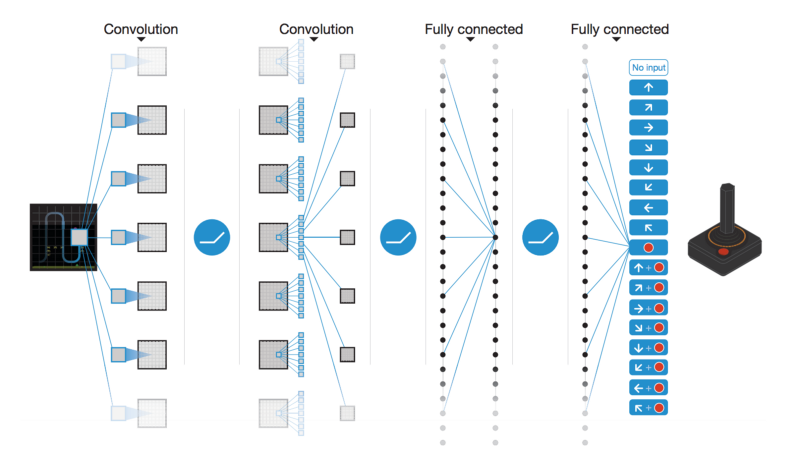
\includegraphics[width=0.8\textwidth]{./figures/deepq.png}
    \caption{ Deep Q-learning Network Illustration \cite{mnih2015human}}
	\label{fig:deepq}
\end{figure}

The massive use of non-linear function approximators for learning value or action-value functions has been depreciated in the past since the convergence is no longer guaranteed, and thus the practical learning tend to be unstable. To search for practical solution, Mnih et al. \cite{mnih2015human} apply large neural networks as function approximators, which is known as Deep Q learning. The motivation is that, in our case with the large state space $\mathcal{S}$ of front images during driving, it is impossible to directly compute $Q$. Alternatively, we can use a deep convolutional network to estimate $Q$.

Figure \ref{fig:deepq} illustrates a model of deep Q learning network \cite{mnih2015human}. The first layers of convolution and max-pooling extracts feature from image input. The following fully-connected layers provide decision on the control of a car. The sample network shown estimates a function $Q : S \rightarrow A^n$, which takes an image input and output the expected reward for all possible actions. In the car simulator environment, the control, which is the steering-angle, is continuous. IN this situation, we discretize the action space into 5 values: $\{-0.7, -0.3, 0, 0.3, 0.7\}$.

One challenge when applying neural networks for reinforcement learning is that most optimization algorithms assume that the training samples are independently and identically distributed (i.i.d.). However, this is no longer the case when exploring sequentially in the car simulation. The sequential actions result in states with strong correlation, which will lead to over-fitting. In our situation, we save a finite set of historical states as tuples $(s_t, a_t, r_t, s_{t+1})$. At each epoch, the latest states and historical states are randomly sampled to form a minibatch, allowing the algorithm to learn across a set of uncorrelated transitions.

\subsubsection{ Deep Deterministic Policy Gradient}

We also use the method of deep deterministic policy gradient \cite{lillicrap2015continuous} to solve the continuous control problem as a comparison to discretizing the action space for ordinary deep Q learning. One major challenge with continuous action space (e.g. steering angle) is exploration. We cannot exhaustively explore Q for every action. Researchers in \cite{lillicrap2015continuous} has proposed to add another neural network to estimate the policy, $\mu^{\prime}(s_t | \theta^{\mu})$, in addition to a neural network estimating $Q(s, a| \theta^Q)$. 




\section{Neural Network Structure}
All of the models use the same convolutional and max-pooling structure for image feature extraction. The decision layers are also similar, with small modifications to fit into different situations.

The neural network architecture we use is described in the following:

\begin{table}[htbp]
\centering
\begin{tabular}{|c|c|c|c|c|}
\hline
Component & Layer & \#Filters & Kernel size & Strides  \\ \hline
\multirow{4}{*}{Encoder} & ConvLayer & 32 & $3 \times 3$ & 1 \\
 & MaxPooling & -  & $2 \times 2$ & 2  \\
 & ConvLayer & 32 & $3 \times 3$ & 2  \\
 & ConvLayer & 32 & $3 \times 3$ & 1  \\
 & MaxPooling & -  & $2 \times 2$ & 2  \\ \hline
\end{tabular}
\caption{Encoder}
\label{table:nn_encoder}
\end{table}

\begin{table}[htbp]
\centering
\begin{tabular}{|c|c|c|}
\hline
Component & Layer & \#Units   \\ \hline
Encoder & \multicolumn{2}{|c|}{shown in table \ref{table:nn_encoder}} \\ \hline
\multirow{3}{*}{Predictor} & FC & 1024  \\
 & FC & 512   \\
 & FC & 25   \\ \hline
\end{tabular}
\caption{Encoder and Predictor}
\label{table:nn_whole}
\end{table}

\subsection{Policy Network}
The same policy network structure is used for supervised CNN and DDPG actor network. A linear layer of ouput size 1 is attached to the predictor, with a sigmoid activation, making the range of output action $(0,1)$. The output is then scaled and moved, making the output $2a + 1$, and the range of output $(-1,1)$, matching the control range of steering angle of the car simulator.
\subsection{State-action-value Network for Discretized Q Network}
The following describes the Q function network used by deep Q learning with discretized action space. A linear layer of output size 5 is attached to the predictor to act as the logits of Q values for 5 discrete actions.
\subsection{State-action-value Network for DDPG Q Network}
The following describes the Q function network used by DDPG state-action-value approximator. The predictor input is modified from 1024 to 1025 to accomodate an extra input of the action value. A linear layer of output size 1 is attached to the predictor to act as the logit of $Q(s,a)$.


\section{Experiment and Performance Evaluation}
\subsection{Supervised CNN}

In supervised learning, we first record a set of images and actions taken by human players on the
simulator. We start the simulator in ``Training mode'' and record all images frames into a local
data folder, along with the statistics of steering angle, speed, throttle. We collect a total
of 7788 image frames. We separate the  data set of images by a training-validation ratio of 4:1. Each image frame is labeled
with the control information of human players and the current speed. To simplify the control, 
we set throttle value constant in our environment, and decide only the steering angle value. Now, a sample of data $(X, y)$ is defined as: $X$
is a image frame, $y$ is the action (steering angle of real value between $-1$ to $1$).

In the data preprocessing part, we transform the original $160 \times 320 \times 3$ image into a gray-scale image of size $80 \times 160$.
The objective is to minimize computation overhead while keeping the most valuable information (removing backgrounds) for control decision.

The structure of the network used for training the supervised model
is refereed to the Nvidia-Net \cite{bojarski2016end}.  To minimize the impact of over-fitting, we a dropout layer with probability $0.5$
after the encoder layers.
We use batch gradient descent and the Adam optimizer with default setting:
$\beta_1=0.9$ and $\beta_2=0.999$. The batch size is $512$.

The loss variation during training process is shown in Figure \ref{fig:loss_curve}. We get a minimal value of validation loss
$0.0181764$
in the iteration number 43. At the same time the loss on training set is $0.0549367$. Model is restored after each epoch. We later use
several models to show the model performance in our video.
An observation is that the loss increases
after epoch 48. The reason may be the neural network has converged to a local minimum and present unstableness.
\subsection{Reinforcement Learning}

The same training and evaluation process is done to both discretized and continuous deep Q learning methods.

The reward is defined as the difference in speed between frame, normalized by time difference between frames. At exploration stage, the car simulator is given random action with normal distribution, with mean $\mu$ as 0 and a very small variance $\sigma$. The reasoning behind is that in the human driving experience, steering angle is 0 in most of the time, and dramatic steering is unnecessary. Discretized deep Q learning also chooses random action from the discretized action space with the same normal distribution. State image, action and reward obtained from the simulator is saved in a replay buffer in memory. Each exploration episode ends when the between-frame speed drop is larger than a constant.

Each exploration episode is followed by a training stage. A training sample of 64 is randomly drawn from the replay buffer. For Q network, the loss function used is ``reduce\_mean'' while the optimizer is ``RMSPropOptimizer''. For actor network of DDPG, the loss function is $-Q(s,\mu(s))$ and the optimizer is a simple ``GradientDescentOptimizer''.

For DDPG, as described in \cite{lillicrap2015continuous}, we created a copy of the two networks as target networks and update them with $\tau = 0.5$. The update happens after each training stage.

After certain exploration-training iterations, the model is evaluated. The model is allowed to drive the simulator with its policy, $\arg\max_aQ(s,a)$ for discretized deep Q learning and target actor network $\mu(s)$ for DDPG. The performance is observed as the time it can stay on track before hitting the same stop criteria of exploration. 

Unfortunately, both methods cannot obtain a self-driving agent with better-than-random driving performance within project timeline. After 24 hours of exploration and training for both models, the models still drives off the track right from the start. The situation persists with different choice of hyper-parameters, such as learning rate of optimizers, update value $\tau$, initializer options and others.

\section{Discussion}

\subsection{Successful Convergence for Supervised CNN}

In the experiment of Supervised CNN agent, we obtained a model that can drive the car simulator to an acceptable stability. We can observe from the video footage of model evaluation that the model can drive the car simulator on track indefinitely, without going offroad. The model drives in a wavy way, turning from left to right and from right to left on a straight road.

Although we obtained a model that can follow a track, the result is far from being transfered to real-world road situation. The most obvious flaw is that the car agent cannot drive in straight line, which is absoultely a requirement for driving in a stable way on road.

However, the success of this experiment shows that using supervised CNN to train a self-driving agent is a viable option. With better human driver experience and larger data samples to learn from, supervised learning can provide a good human driving approximation.

\subsection{Failure in Reinforcement Learning Lethods}

There are a number of factors that might contribute to the failure of using reinforcement learning methods in our context.

\subsubsection{Very large state space}

The state space of the self-driving problem is too large for reinforcement learning methods to explore. The state is a 320 $\times$ 160, 24-bit color RGB image, captured from a 3-dimensional game environment that is dedicated to simulate real-world environment. The large state space makes it difficult and time consuming for the reinforcement learning exploration to sufficiently explore the state space. 

Comparing our result with the success of Deep Mind in applying deep Q algorithm in Atari games \cite{mnih2013playing}, we would suggest that Atari games have a less complex, 2-dimensional environment, which makes variation between images and the state space much smaller.

\subsubsection{Long training time}

In the experiment of DDPG, the training of 64 samples takes 30 seconds in average, and the updating of target networks takes another 30 seconds. Ignoring exploration, 230400 samples can be trained in 24 hours. Having a long training time makes it hard to observe inability in convergence and hyper-parameter tuning.

\subsection{Possible Improvements}

\subsubsection{Asynchronous Training and Exploration}

Exploration and training can be made parallel as they are not in conflict. This saves some time in exploration and data collection.

\subsubsection{Sharing weights for convolutional layers}

Convolutional layers serves as feature extractor in the network. In DDPG, weights of those layers can be shared between the target networks and the training networks, and between Q networks and actor networks. This can save time in training and updating of networks.


\section{Workload distribution}
\begin{table}[htbp]
\centering
\begin{tabular}{|c|c|c|}
\hline
Student name & Student ID & Task workload   \\ \hline
Hok Chun Ng & 20272532 & Information search and Implementation for DDPG Q Network \\
Shengyuan Zhang & 20565161 & Information search and Implementation for Discretized Q Network   \\
Ge Chen & 20360858 & Information search and Implementation for Supervised Model \\ \hline
\end{tabular}
\label{table:task_allocation}
\end{table}

\section{Link to Video and Code}
Links

Video:
\begin{verbatim}
    https://youtu.be/pGNKSOzXNyI
\end{verbatim}

Github Code Repo: 
\begin{verbatim}
    https://github.com/princhenee/comp5212_2018_pp
\end{verbatim}


% \begin{figure}
% \centering
% \includegraphics[width=0.3\textwidth]{frog.jpg}
% \caption{\label{fig:frog}This frog was uploaded to writeLaTeX via the project menu.}
% \end{figure}

\bibliography{ref}{}
\bibliographystyle{plain}
\end{document}
